%% -----------------------------------------------------------------
%%  Original Template
%% -----------------------------------------------------------------
%%
%%   Author:    Tim Callagha, University of Tasmania (UTas)
%%   Email:     tgc@hilbert.maths.utas.edu.au
%%   Copyright: 2003 Tim Callagha
%% 
%%   Style file to assist in generating a University of Tasmania PhD thesis
%%   in Mathematics. Contains all the required formatting options and 
%%   header/footer information that is set out in the Research Higher Degrees 
%%   Resource Handbook (2003 version)
%%
%%   This file should be easily modifiable to comply with
%%   minor formatting changes (such as the left margin width etc.)
%% 
%%   This style file is designed primarily for students of mathematics at UTas who
%%   are undertaking a PhD. However, only very minor changes need to be made to the 
%%   wording in a few places to use it as a template for an honours or Masters thesis 
%%   as well. In fact, there is no particular reason why this could be not used for, 
%%   say, an Arts thesis (Shock, Horror!) since it is mainly about the formatting and 
%%   less about the content. However, the heading and chapter structure has been chosen
%%   so as to be more in line with standard practice in the scientific streams. Again, 
%%   if you know what you're doing then it's really not that difficult to modify the style 
%%   file at the appropriate places. I have tried to comment it quite heavily so that 
%%   interested persons can see how it does all its work and, hopefully, make changes 
%%   that reflect personal tastes etc.
%%
%%   Source: http://staff.acecrc.org.au/~mdsumner/TCallaghan/
%% 
%%   This work consists of the files listed in the README file.
%%
%% -----------------------------------------------------------------
%%  Modifications for Australian Maritime College (AMC) and
%%	University of Tasmania (UTas) Department of Engineering 
%% -----------------------------------------------------------------
%%
%%   Author:  Konrad Zürcher, Australian Maritime College (AMC)
%%   Email:   Konrad.Zurcher@utas.edu.au
%%   License: MIT License
%%
%%	 Modified version of the original template adjusted for styling
%%   requirements of the University of Tasmania (UTas) Department of 
%%   Engineering and the Australian Maritime College (AMC).
%%
%%   GitHub: https://github.com/SeaShadow/LaTeX-AMC-PhD-Template
%% 
%%   This work consists of the files listed in the README file.
%%
%% -----------------------------------------------------------------
%%

% thesis.tex (starting point of a UTas mathematics thesis)

% Note that the following defaults are also contained in the 'report' class
% (this is not exhaustive...see appropriate references for all options)
% 'oneside' mode...overide with 'twoside' to force output for two-sided printing.
% 'final' mode...overide with 'draft' to see linebreak malfunctioning.
% For example, to use two-sided printing one would declare the 'documentclass'
% as follows...
% '\documentclass[11pt,a4paper,twoside]{report}'
%
% Specific Mathematical options are as follows
% 'leqno' to force equation numbering on the left side of the page.
% 'fleqn' to force formulas to flush left (centered is the default).
% If 'fleqn' is specified then the left indent is controlled with '\mathindent'.
% i.e. '\setlength{\mathindent}{2.5cm}'

% Declare overall type of document (use 11pt report class on A4 paper).
\documentclass[11pt,a4paper,draft]{report}

% If you want to generate an index you should include the following command
% which puts a makeindex command in the preamble. Additionally, you need to un-comment
% the file 'index' in the '\includeonly' command below and also include the 'index'
% file in the main document.
\makeindex
\PassOptionsToPackage{nottoc}{tocbibind}

% Include the style file which contains all the required formatting
% information that is set out in the Research Higher Degrees Resource
% Handbook (2003 version). NOTE: This file uses the following packages
% 'graphicx' for graphics manipulation
% 'fancyhdr' for nice headers and footers.
% 'makeidx' for generating the index
% 'tocbibind' for adding table of contents entries for bibliography, index etc.
% 'sectsty' for generating stylised chapter and section headings.
% 'lipsum' for generating dummy text.
% 'natbib' and 'har2nat' for bib citations.
% 'xcolor' color package.
% 'epstopdf' EPS to PDF conversion.
% You will need to make sure your LaTeX installation has these packages
% installed...else it wont work :(
\usepackage{Packages/mathphdthesis}

% Here you would include any additional packages that you want to use.
% You should make sure they don't clash with the above packages that
% are in use in the style file.

% Specify which pieces (other .tex files) you plan to include. You can comment
% out files that you will include later or have already finished to speed
% up TeX processing
\includeonly{
Frontbackmatter/prelude 	% Contains all the relevant candidate information (name, degrees, abstract etc)
,Frontbackmatter/newcom 	% Place all you new commands in here
,Nomenclature/nomenclature  % The nomenclature chapter
,Chapters/Intro/intro  	    % The first chapter
,Appendices/app0   			% Needed to switch to appendix mode
,index  					% Places the index in the thesis
}

% Begin the thesis
\begin{document}

% Include all the pieces of your thesis in here
% prelude.tex (specification of which features in `mathphdthesis.sty' you
% are using, your personal information, and your title & abstract)

% Specify features of `mathphdthesis.sty' you want to use:
\titlepgtrue 												% Main title page (required)
\signaturepagetrue 											% Page for declaration of originality (required)
\copyrighttrue 												% Copyright page (required)
\abswithesistrue 											% Abstract to be bound with thesis (optional)
\acktrue 													% Acknowledgments page (optional)
\tablecontentstrue 											% Table of contents page (required)
\tablespagetrue 											% Table of contents page for tables (required only if you have tables)
\figurespagetrue 											% Table of contents page for figures (required only if you have figures)

% Title, author, supervisors, university, date of submission
\title{Modelling of sandwich plates and piezoelectric transducers to identify the severity of mechanical damage}							% Thesis title
\author{Piotr Fiborek} 	% First name and surname of candidate (e.g. John Doe)
\prevdegrees{M.Sc. Eng.}              			% Specify your previous degrees (e.g. B.E. (Hons))
\institute{Mechanics of Intelligent Structures Department}								% Institute of department (e.g. National Centre for Maritime Engineering and Hydrodynamics)

\submittedfor{A dissertation submitted to the Scientific Board of the Szewalski Institute of Fluid Flow Machinery, Polish Academy of Sciences in partial fulfillment of the requirements for the Degree of Doctor of Philosophy}			% Degree thesis is submitted for (e.g. Submitted in fulfillment of the requirements for the Degree of Doctor of Philosophy)
\advisor{ Pawe\l{} Kudela, D.Sc. Ph.D. Eng.} % Supervisors: (e.g. Prof. Lawrence K. Forbes)
\dept{The Szewalski Institute of Fluid Flow Machinery, Polish Academy of Sciences}
\submitdate{June, 2022}						% Month & year of your thesis submission (e.g. January, 2016)

% Abstract to be bound with thesis
\newcommand{\abstextwithesis}
{
%Basic abstract goes here. Can use paragraphs and normal \LaTeX commands.
...
}

% Acknowledgments page
\newcommand{\acknowledgement}
{
}

% Engineering guote page
\newcommand{\engineeringquote}
{
\null\vskip1.8in
\begin{quote}
"Engineering ."\begin{flushright}- aaa 
\end{flushright}
\end{quote}
}

% Bibliography Title
\renewcommand{\bibname}{Bibliography}
% Bibliography spacing
\setlength\bibitemsep{1.5\itemsep}

% Settings for array package
\newcolumntype{L}[1]{>{\raggedright\let\newline\\\arraybackslash\hspace{0pt}}m{#1}}
\newcolumntype{C}[1]{>{\centering\let\newline\\\arraybackslash\hspace{0pt}}m{#1}}
\newcolumntype{R}[1]{>{\raggedleft\let\newline\\\arraybackslash\hspace{0pt}}m{#1}}

% Take care of things in `mathphdthesis.sty' behind the scenes.
% Basically just does a check of all the fields that have been activated
% above and fills out the appropriate pages and adds them to the thesis.
\beforepreface
\afterpreface

% newcom.tex (new command definitions)

% Some examples (yours may be different):
\newtheorem{theorem}{Theorem}[section]
\newtheorem{lemma}[theorem]{Lemma}
\newcommand{\bfx}{{\ensuremath{\mathbf{x}}}}

% chap9.tex (Chapter 9 of the thesis)

%\chapter[NOMENCLATURE]{NOMENCLATURE}
% Overwrite TOC chapter title
\chapter*{NOMENCLATURE}
\addcontentsline{toc}{chapter}{NOMENCLATURE}
\label{nomenclature}

% -----------------------------------------------------------------------------------------------------------------
% Greek symbols
% -----------------------------------------------------------------------------------------------------------------

% GENERAL CONSTANTS

% -----------------------------------------------------------------------------------------------------------------
% Dimensionless numbers
% -----------------------------------------------------------------------------------------------------------------


% -----------------------------------------------------------------------------------------------------------------
% Roman symbols
% -----------------------------------------------------------------------------------------------------------------

% AREAS 
% DIMENSIONS
\printnomenclature[6em]
%\printnomenclature[2cm]

% Set page numbering to arabic the first time we commence a chapter.
% This is required to get the page numbering correct.
\pagenumbering{arabic}

% Note that the text in the [] brackets is the one that will
% appear in the table of contents, whilst the text in the {}
% brackets will appear in the main thesis.

%% CHAPTER HEADER /////////////////////////////////////////////////////////////////////////////////////
\chapter[Introduction]{Introduction}
\label{ch:intro}
The dissertation is the result of the author’s work as an assistant in the Department of Mechanics of Intelligent Structures, Institute of Fluid Flow Machinery, Polish Academy of Sciences.
Most of the work was carried out within the framework of a research project titled ‘Model-assisted damage identification function for Structural Health Monitoring of composite structures under a varied environmental condition', which was granted to the author by the National Science Centre, Poland.
The primary objective was to develop a new approach to a sandwich structure assessment based on guided waves techniques under varied operating conditions.
The essence of the proposed method was to establish an accurate and numerically efficient model of the wave propagation in the sandwich structure, which allowed for determining the mechanical damage severity.
A better understanding of guided wave behaviour in such structures and their interaction with damage may allow the development of more precise structural health monitoring strategies, reducing costs without compromising the safety of the liable systems.
%% CHAPTER INTRODUCTION ///////////////////////////////////////////////////////////////////////////////

%% INCLUDE SECTIONS ///////////////////////////////////////////////////////////////////////////////////
%% SECTION HEADER /////////////////////////////////////////////////////////////////////////////////////
\section{Sandwich Composite Structures}
\label{sec:scs}

%% SECTION CONTENT ////////////////////////////////////////////////////////////////////////////////////
Composites consist of two or more different materials, such as plastics, resins, metal alloys, glass, carbon or bio-based fibres. The combination of material constituents gives  structure benefits from the properties of the component materials, e.g., the strength of carbon fibres and the low density of the polymer resin in the case of \ac{cfrp}.
The contribution of lightweight composite materials to the production of structural components has been increasing rapidly since the middle of the last century.
Due to the high strength-to-weight ratio, higher operating temperatures, greater stiffness and higher
reliability, composite materials are extensively used in the aircraft and aerospace industry and civil constructions.
Composites account for more than 50\% of the total weight of the aircraft Boeing B787 and Airbus A350 \cite{giurgiutiu2015structural}.

One group of composites includes sandwich panels, which is a type of multi-layered structure that are composed of the mid-core sandwiched between thin skins.
The skins, made of high strength materials, are designed to carry tensile or compressive stresses from longitudinal forces and bending moments.
On the other hand, the core transmits mainly shear stresses from transverse forces.
It also separates the skins, which increases structural stiffness for thin layers, improves insulation properties, and reduces weight while maintaining strength properties similar to the solid construction of the same density.
A popular core used in engineering structures is a honeycomb geometry core.
Fig.~\ref{fig:hcp} shows the construction of the \ac{hsc}.
The core can be made of aluminium, cardboard or Nomex. 
\begin{figure}[H] %hbtp
	\begin{center}
		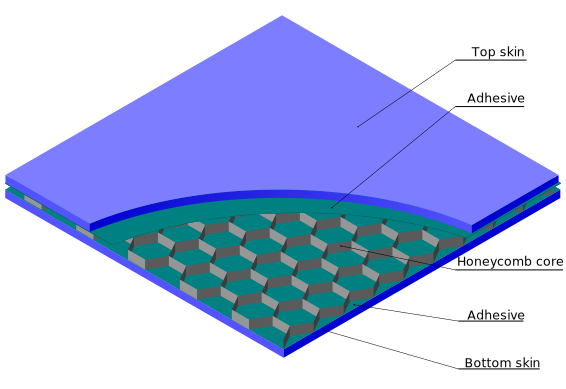
\includegraphics{Intro/honeycomb_plate}
		\caption{
			\label{fig:hcp} Structure of the honeycomb sandwich composite.}
		\vspace{-0.5cm}
	\end{center}
\end{figure}

However, these complex structures are exposed to various types of damage that are not found in metal alloy materials, e.g., hidden disbonds between the skin and the core, delamination of the composite skins, or the core impact damage.
They can occur either during a manufacturing process, storage or in-service life.
Therefore, advanced methods are required for online damage detection.
Thus, the use of composites has forced the development of advanced approaches to structural inspections, e.g., methods based on elastic wave propagation had to account for the anisotropic structure of the material.
%% SECTION HEADER /////////////////////////////////////////////////////////////////////////////////////
\section{Structural health monitoring}
\label{sec:scm}

%% SECTION CONTENT ////////////////////////////////////////////////////////////////////////////////////
\Ac{shm} is the process of implementing an advanced damage identification strategy for structural or mechanical systems \cite{farrar2007introduction}.
The \ac{shm} systems usually consist of a sensor network, a \ac{dau}, and a central processor.
The \ac{dau} is responsible for collecting the data measured by the sensor network.
A central unit then determines the current state of the structure through signal processing and statistical classification.
The implementation of \ac{shm} aims to extend the safe life of the monitored system, or usage of lightweight materials, which leads to cost reduction in production and operation.
For example, composites and adhesive bonding techniques reduces the aircraft's overall weight, reducing fuel consumption \cite{scelsi2011potential}.
\ac{shm} is most commonly found in structures, such as aerospace, civil and mechanical engineering, where damage can have catastrophic consequences.

Rytter, in his dissertation \cite{rytter1993vibrational}, classified the \ac{shm} system advancement into the following four levels:
\begin{itemize}
	\item[] \textbf{Level 1}: Detection.
	\item[] \textbf{Level 2}: Localization.
	\item[] \textbf{Level 3}: Assessment.
	\item[] \textbf{Level 4}: Consequence.
\end{itemize}
The first level determines if any adverse change in the geometric has occurred or material characteristics of the system. The second level leads to the localization of the damage.
The third and fourth level systems determine the size of the flaw and decide whether any maintenance is necessary, respectively.
The existence and location of faults can be defined in unsupervised learning mode by taking a threshold value for a measurable, damage-sensitive system feature. The threshold should be compensated depending on the prevailing operational and environmental conditions.
In contrast, damage size is determined in supervised learning mode based on an analytical model or data extracted experimentally from the structure \cite{worden2007fundamental}.
%% SECTION HEADER /////////////////////////////////////////////////////////////////////////////////////
\section{Piezoelectric Transducers}
\label{sec:challenges}

%% SECTION CONTENT ////////////////////////////////////////////////////////////////////////////////////


%% SECTION HEADER /////////////////////////////////////////////////////////////////////////////////////
\section{Chosen \ac{shm} techniques using \acp{pzt}}
\label{sec:techniques}

%% SECTION CONTENT ////////////////////////////////////////////////////////////////////////////////////

\subsection{Guided waves based techniques}


\Acp{gw} are mechanical vibrations being a superposition of shear and longitudinal waves propagating in a bounded elastic medium, e.g., bars, beams, rods, plates and shells. 
Guided waves are multi-modal and dispersive, i.e. more than one mode travels simultaneously through the medium with the phase velocity depending on the frequency.
Fig.~\ref{fig:dispersion} shows an example of dispersion curves generated by the Dispersion Calculator~\cite{huber2021dispersion} software tool for a 1 mm thick \ac{cfrp} plate in the frequency range 0-2000 kHz.
\Ac{a0} and \ac{s0}, considering the distribution of particle displacements on the upper and lower free surface relative to a central surface, are observed for low frequencies.
The mode shapes are pictured in Fig.~\ref{fig:mode_shape}, with the \ac{s0} particle displacements being dominant in-plane, while the \ac{a0} is dominated by out-of-plane.
Moreover, higher harmonic modes appear over the cut-off frequency, as shown in Fig.~\ref{fig:dispersion}.
\begin{figure}
	%	\begin{center}
	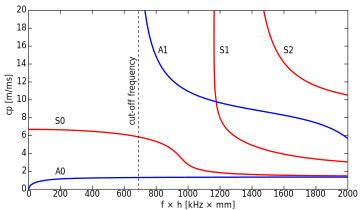
\includegraphics[width=1\linewidth]{Intro/dispersion}
	%	\end{center}
	\caption{Dispersion diagram for a 1 mm \ac{cfrp} plate (adopted from Dispersion Calculator~\cite{huber2021dispersion}). Red and blue solid curves represent symmetric and antisymmetric modes, respectively; a black dashed line indicates the cut-off frequency for higher modes.}
	\label{fig:dispersion}
\end{figure}
\begin{figure}
	%	\begin{center}
	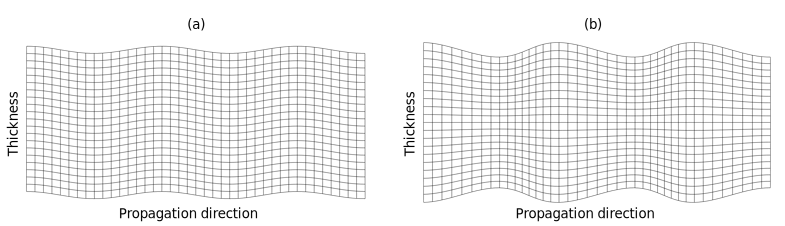
\includegraphics[width=1\linewidth]{Intro/mode_shape}
	%	\end{center}
	\caption{Mode shape of the \textbf{(a)} \ac{a0} and \textbf{(b)} \ac{s0} at 100 kHz for \(\phi=0^{\circ}\) in 2 mm composite plate (exported from Dispersion Calculator~\cite{huber2021dispersion}).}
	\label{fig:mode_shape}
\end{figure}

Detection schemes based on \acp{gw} exploit reflection, attenuation, and mode conversion when the propagating wave encounters a discontinuity in the structure \cite{alleyne1992interaction}.
Thus, this technique is efficient in detecting various types of defects, such as delamination \cite{sohn2011delamination,tian2015delamination}, adhesive disbonds \cite{rucka2018damage,balasubramaniam2021ultrasonic}, corrosion changes \cite{alleyne1995long,lowe1998defect}, cracks \cite{tua2004detection,lu2006crack,zima2020detection} and failures occurring in \acp{hsc} \cite{mustapha2011assessment, sikdar2016guided, sikdar2016ultrasonic,radzienski2016assessment, yu2019core}.
Many techniques based on \ac{gw} propagation have been developed for damage detection and localization.
A pitch-catch technique \cite{ihn2008pitch, sikdar2017structural} uses a pair of detached sensors, one excites, and the other receives a signal.
If the wave encounters a defect between the sensors, it will scatter, and the recorded signal will be distorted.
In the case of the pulse-echo technique \cite{guo1993interaction, kudela2008damage}, there is one sensor that excites the wave and, at the same time, registers possible echoes from the damage.
The damage localization can be determined if the wave speed is known and the time of flight is measured.
The radar principles were utilized in a phased array technique for plate inspection \cite{giurgiutiu2004embedded, ostachowicz2008elastic, kudela2018structural}.
The technique uses an array of transducers, each excited with an appropriate time offset, to focus all the waves at a single grid point of the area to be inspected.
A damage map is determined once the signals are obtained and processed for the entire grid.
Fink proposed a different approach, developing what he called a time-reversal mirror \cite{fink1992time}.
In this method, the wave propagates from one sensor to another, and then after time-reversal and dispersion compensation, the wave is re-emitted to the origin sensor.
The resulting signal will be a mirror image of the forcing signal only if the wave does not encounter damage along the way \cite{park2007time, eremin2016analytically}.

The \acp{pzt} can be used mutually as actuator-receiver pairs or as a single actuator with other types of devices, e.g. \ac{sldv}, \ac{fbg} sensors.
The \acp{pzt} generate high forces with broadband frequency, so methods based on \ac{gw} can detect various damage types of different sizes in a large inspected area.
Moreover, specific algorithms do not require a baseline model, and the method implementation is economically efficient.

\subsection{Electromechanical impedance methods}
\Ac{emi} spectroscopy is also an effective and powerful technique in \ac{shm} for real-time structural damage assessment \cite{park2003overview}.
The basis of this method is the influence of the mechanical impedance of the inspected host structure on the electrical impedance of the \ac{pzt} attached to the structure.
Assuming that the mechanical property of the sensor remains unchanged over the monitoring period, any changes in measurements of the electrical impedance can be considered a difference in the structure stiffness, which in turn can indicate that a defect has occurred.

Fundamentals of the \ac{emi} method were introduced by Liang et al. \cite{liang1994impedance}.
An analytical model of a \ac{pzt} actuator bonded to one end of a single degree of freedom mass-spring-damper system was presented in this pioneering work.
In the early papers, the authors adopted quasi-static sensor approximation until  Giurgiutiu and Zagrai \cite{giurgiutiu2000characterization} derived an expression where the sensor dynamic was incorporated.
The dynamics of a single \ac{pzt} with various boundary conditions (free, clamped and elastically constrained) and sensor attached to a beam were considered.
Further investigation was performed for the sensor bonded to the host structures was performed \cite{zagrai2001electro, giurgiutiu2005damage}.
Damage detection is realized by comparing the state of the structure with the reference state using overall statistical damage indices, e.g., the \ac{rmsd}, the \ac{mapd}, \ac{ccd} and \ac{pnn}.
Malinowski et al. \cite{malinowski2014characterisation, malinowski2015use} investigated the effects of \ac{emi} changes related to the state of the adhesive layer between two composite plates.
The technique has been used to evaluate weak bonds due to inadequate adhesive curing temperature, release agent and moisture contamination. This type of damage is not detectable using the method based on \ac{gw} propagation.
Experimental testing was conducted on weakened samples and compared with a reference.
The \ac{rms} of the conductance in the range of 3-5 MHz and the first thickness resonant frequency shift were considered for bond-line assessment.

An and Sohn \cite{an2012integrated} proposed a new damage detection technique that combines \ac{emi} and \ac{gw} advantages.
In the method, measured admittance characteristic is separated into two parts: active and passive.
\Ac{di} is a weighted sum of two indicators obtained from \ac{gw} signal and active admittance.
Because passive impedance is only sensitive to temperature variation, it is used for temperature compensation on both mentioned signals.
Instead of two \acp{di}, Sevillano et al. \cite{sevillano2016damage} proposed more integrated \ac{di} based on the electromechanical power dissipation of the \ac{pzt} sensor.

The \ac{emi} technique can detect damage, such as delamination or cracks, but is also sensitive to changes, such as weak bonds, which the \ac{gw} method is ineffective at detecting.
However, the \ac{emi} is a local method for the high frequency.
Giurgiutiu et al. \cite{giurgiutiu2001electro} obtained consistent results for crack detection in distances up to 40 mm in the frequency range 300-450 kHz. 
This method is also sensitive to environmental conditions such as temperature and humidity fluctuations\cite{bhalla2002practical} or loading variations \cite{lim2011impedance}.

%\subsection{Modal analysis techniques}
\input{Chapters/Intro/sec:chall2enges}

\section{Conclusions}
\label{sec:conclusionsIntro}

%% SECTION CONTENT ////////////////////////////////////////////////////////////////////////////////////
The Introduction briefly reviewed issues raised in the dissertation, i.e., composite materials, their construction and applications; definition of the \ac{shm} and application of the \ac{pzt} sensors in damage detection; and challenges in \ac{gw} propagation modelling for damage severity assessment in \acp{hsc}.

According to the literature review, a useful method for damage size assessment in \ac{hsc} is needed to enhance the safety of using composite structures.
In the dissertation, a novel approach for assessing the size of mechanical damage in a sandwich panel was proposed and developed using a \ac{gw} propagation technique.
This procedure involved actuation of elastic waves in the investigated structure, as well as their recording with the use of the \ac{pzt} setup.
The signals and a preliminary numerical analysis that defined a function of the impact of damage on wave propagation were used to estimate the defect severity.
The milestone of the dissertation was to prepare numerically effective model of \ac{gw} propagation in a sandwich panel.
The selection process of a suitable numerical modelling technique addressed the following issues:
\begin{itemize}
	\item flexibility to model the complex structure of the honeycomb core
	\item time efficiency due to the large number of \ac{dof} in the model
	\item possibility of parallel calculation on the \ac{gpu}.
\end{itemize}
% Note that the text in the [] brackets is the one that will
% appear in the table of contents, whilst the text in the {}
% brackets will appear in the main thesis.

%% CHAPTER HEADER /////////////////////////////////////////////////////////////////////////////////////

%% CHAPTER INTRODUCTION ///////////////////////////////////////////////////////////////////////////////

\appendix
%% INCLUDE SECTIONS ///////////////////////////////////////////////////////////////////////////////////
% Note that the text in the [] brackets is the one that will
% appear in the table of contents, whilst the text in the {}
% brackets will appear in the main thesis.

%% APPENDIX HEADER ////////////////////////////////////////////////////////////////////////////////////
\chapter{Elementary matrices of the equation of motion.}
\label{app:matrices}
%% APPENDIX CONTENT ///////////////////////////////////////////////////////////////////////////////////

\section{\ac{pzt} matrices}
% start a new page without indent 4.6cm
%\clearpage
The effective properties of the \ac{cfrp} and homogenized honeycomb core are given in Tab.~\ref{tab:properties_eff}.
\vspace{-12pt}
\begin{table}[H]
	%	\centering
	\small
	
	\tabcolsep=0.25cm
	\caption{\label{tab:properties_eff} The effective mechanical properties.}
	\begin{tabular}{ccccccccc}
		\toprule
		\multirow{2}{*}{\textbf{Material}} & $\boldsymbol{E_{11}}$ & $\boldsymbol{E_{22}}$ & $\boldsymbol{E_{33}}$ & $\boldsymbol{G_{12}}$ & $\boldsymbol{G_{23}}$ & $\boldsymbol{\nu_{12}}$	& $\boldsymbol{\nu_{23}}$ & $\boldsymbol{\rho}$ \\
		& \textbf{[GPa]} & \textbf{[GPa]} & \textbf{[GPa]} & \textbf{[GPa]} & \textbf{[GPa]} & \textbf{[--]} & \textbf{[--]} & \textbf{[kg/m}$\boldsymbol{^3}$\textbf{]}\\
		\midrule
		\ac{cfrp} & 137 & 8.7 & 8.7 & 3.61 & 3.19 & 0.28 & 0.37 & 1569\\
		single layer & & & & & & & &\\ \midrule
		aluminium & 40e{$-$6} & 40e{$-$6} & 663e{$-$3} & 24e{$-$6} & 148e{$-$3} & 0.998 & 0.02e{$-$3} & 25.36\\
		honeycomb & & & & & & & &\\
		\bottomrule
	\end{tabular}
\end{table}

% Note that the text in the [] brackets is the one that will
% appear in the table of contents, whilst the text in the {}
% brackets will appear in the main thesis.

%% APPENDIX HEADER ////////////////////////////////////////////////////////////////////////////////////

\chapter{Interfaces coupling matrix}
\label{app:algorithm}

%% APPENDIX CONTENT ///////////////////////////////////////////////////////////////////////////////////
% Note that the text in the [] brackets is the one that will
% appear in the table of contents, whilst the text in the {}
% brackets will appear in the main thesis.

%% APPENDIX HEADER ////////////////////////////////////////////////////////////////////////////////////
\chapter[Appendix 3]{Appendix 3}
\label{appc}

%% APPENDIX CONTENT ///////////////////////////////////////////////////////////////////////////////////

\lipsum[1]


% A small file that prints the index in the main document.
% No need to alter this file...
\printindex


% Bibliography
\addcontentsline{toc}{chapter}{References/Bibliography}
\printbibliography

\end{document}
